\documentclass[num=11,duedate=04-21-21,course=Algebra\ II,proflastname=Walton]{hwtemplate}

%%% Options for hwtemplate.cls:
%
%% Required:
%
% num - Assignment number
% course - Name or course ID
% proflastname - Last name of professor
% duedate - date that homework is due, in mm-dd-yy
%
%% Optional:
%
% type - type of document (default: Homework)
% studentid - student id used for emails etc. (default: gjg3)
% name - your full name (default: Gabriel Gress)
% emaildomain - domain of email (default: rice.edu)
%
%%%

\begin{document}

\lstset{language=Matlab,%
	%basicstyle=\color{red},
	breaklines=true,%
	morekeywords={matlab2tikz},
	keywordstyle=\color{blue},%
	morekeywords=[2]{1}, keywordstyle=[2]{\color{black}},
	identifierstyle=\color{black},%
	stringstyle=\color{mylilas},
	commentstyle=\color{mygreen},%
	showstringspaces=false,%without this there will be a symbol in the places where there is a space
	numbers=left,%
	numberstyle={\tiny \color{black}},% size of the numbers
	numbersep=9pt, % this defines how far the numbers are from the text
	emph=[1]{for,end,break},emphstyle=[1]\color{red}, %some words to emphasise
	%emph=[2]{word1,word2}, emphstyle=[2]{style},
}

% \lstinputlisting{foo.m}

\maketitle

Collaborated with the Yellow group.

\pagebreak
\problem[1]
\begin{claim} % D-F Exercise 14.2 #3
	Determine the Galois group of \(f(x) = (x^2-2)(x^2-3)(x^2-5)\). Determine all the subfields of the splitting field of this polynomial. Write down the corresponding lattice of Galois groups.
\end{claim}

\begin{proof}
	The roots of \(f\) are \(\left\{ \pm \sqrt{2} , \pm \sqrt{3} , \pm \sqrt{5}  \right\} \). There are no repeated roots and so \(f\) is separable, hence the splitting field over \(f\) is a Galois extension. Thus the Galois group is
	\begin{align*}
		\textrm{Aut}(\Q(\sqrt{2} ,\sqrt{3} ,\sqrt{5} ) / \Q).
	\end{align*}
	Of course the automorphisms must send each root to either itself or its corresponding negative root. Hence the Galois group is given simply by
	\begin{align*}
		\Z_2 \times \Z_2 \times \Z_2.
	\end{align*}
	The subfields of the splitting field are then
	\begin{align*}
	\Q,\; \Q(\sqrt{2} ),\; \Q(\sqrt{3} ),\;\Q(\sqrt{5} ),\; \Q(\sqrt{2} ,\sqrt{3} ),\; \Q(\sqrt{2} ,\sqrt{5} ),\; \Q(\sqrt{3} ,\sqrt{5} ).
	\end{align*}
	The lattice is given below:

	\scalebox{0.12}{
	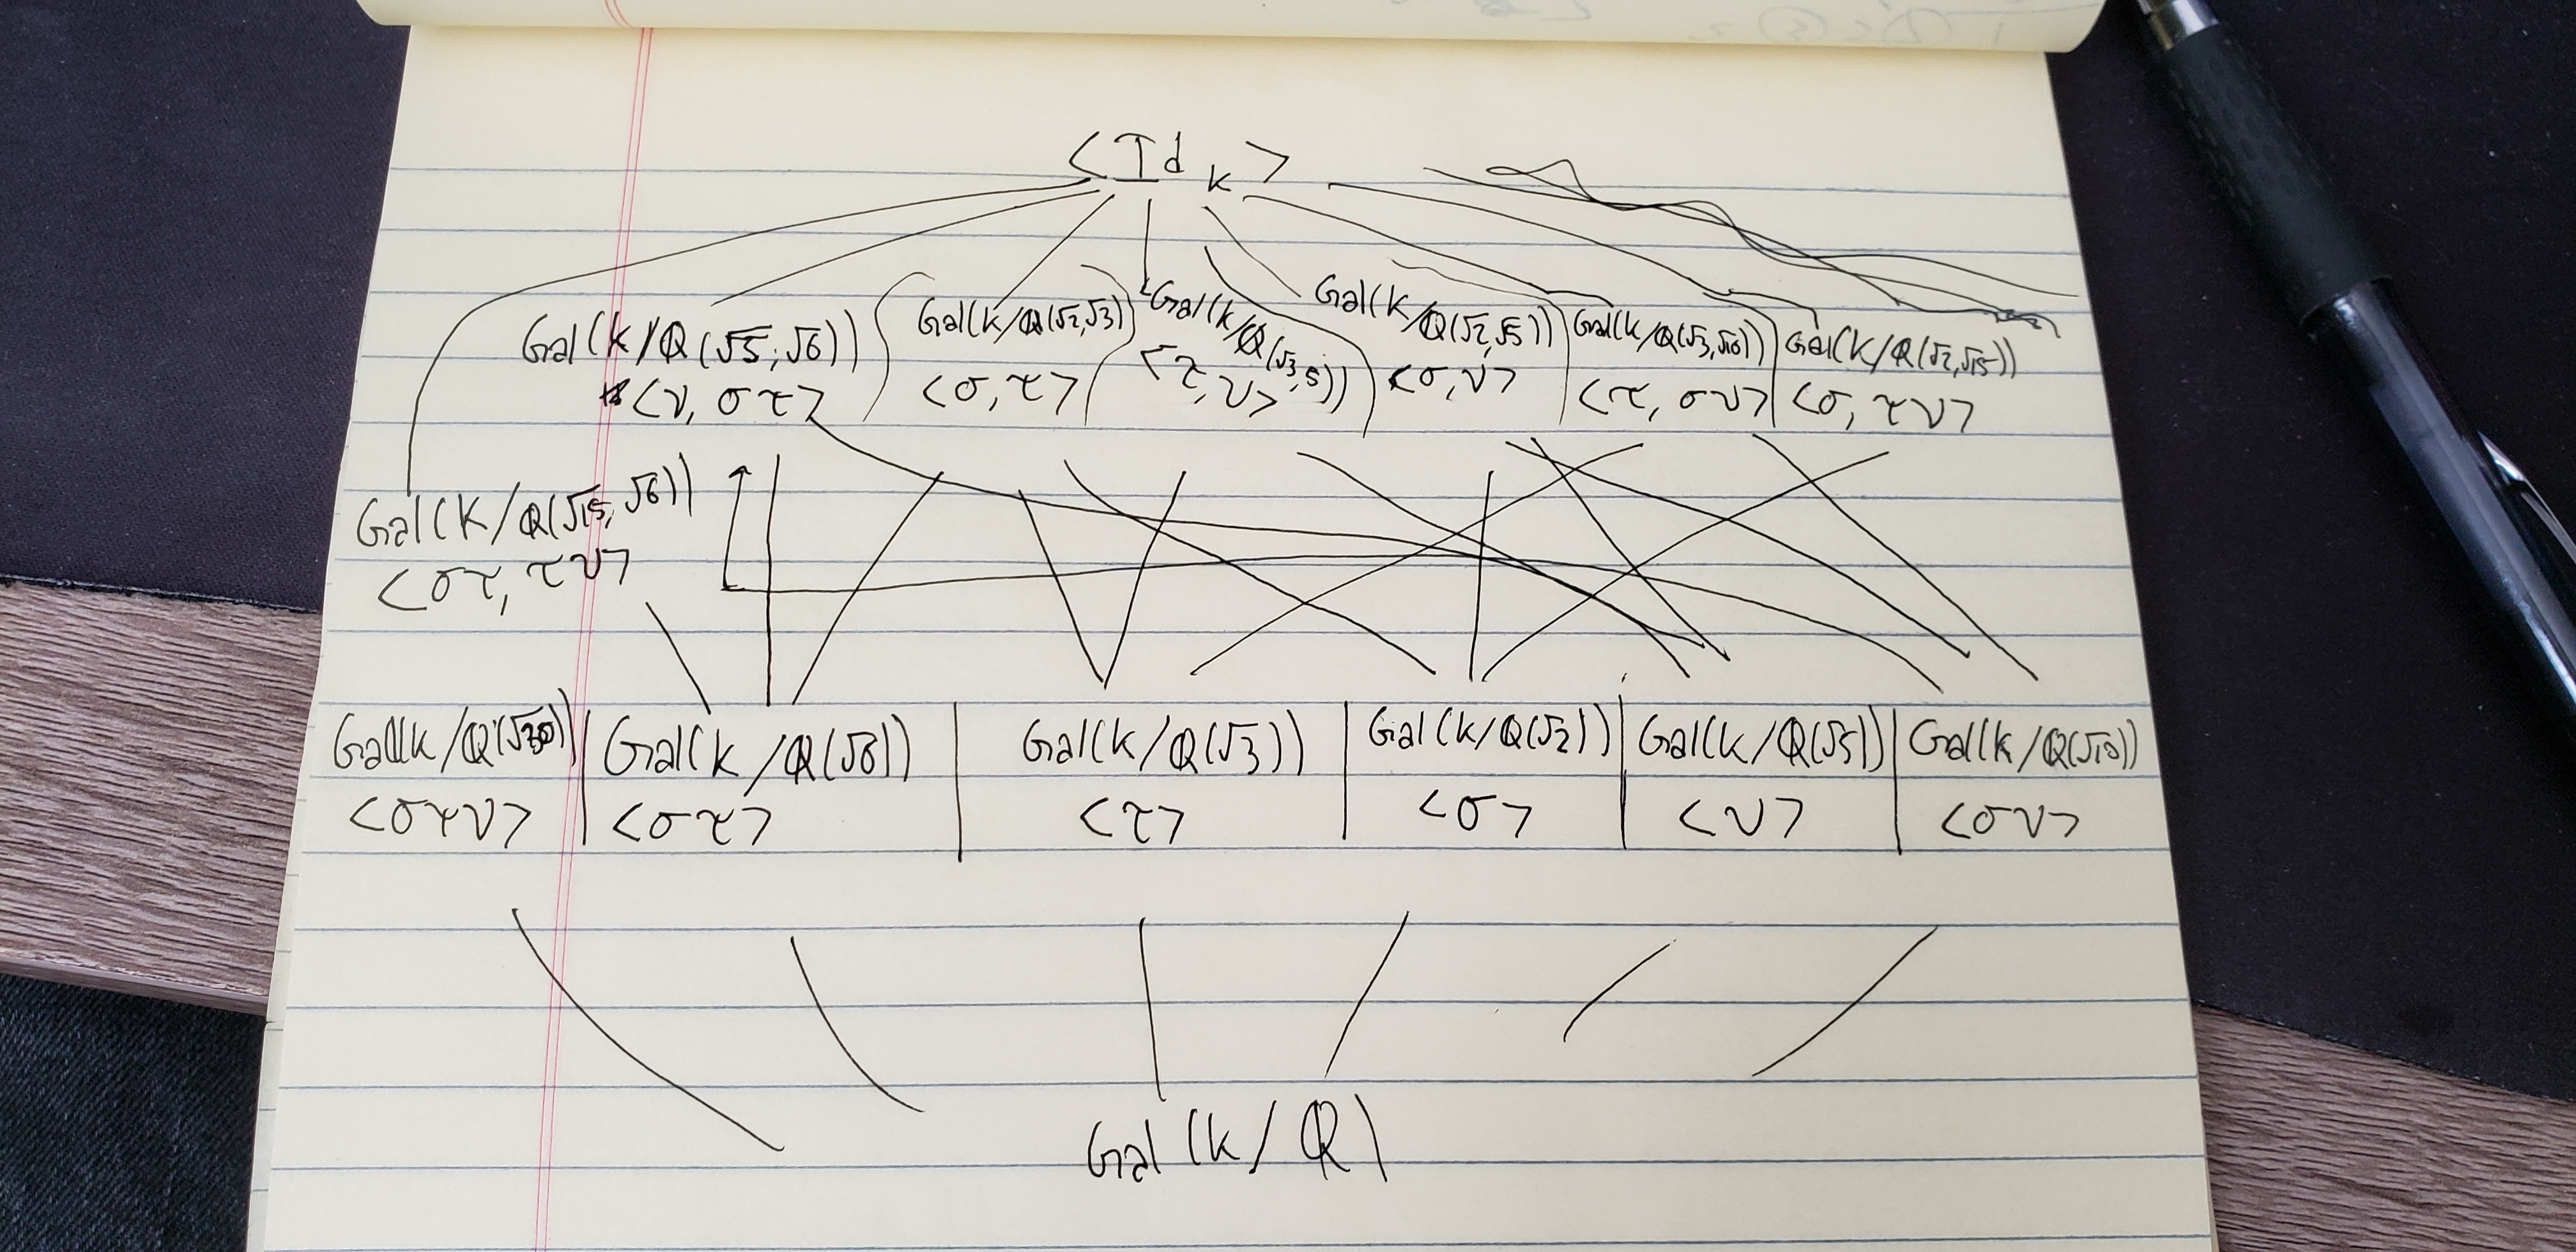
\includegraphics{./figures/lattice.jpg}}
%\begin{figure}[ht]
%    \centering
%     \def\svgwidth{1\linewidth}
%     \input{./figures/lattice.pdf_tex}
%    \caption{Lattice}
%    \label{fig:lattice}
%\end{figure}
\end{proof}

\problem[2]
\begin{claim} % D-F Exercise 14.2 #6
	Let \(K = \Q(\sqrt[8]{2} ,i)\) and let \(F_1 = \Q(i), F_2 = \Q(\sqrt{2} ), F_3 = \Q(\sqrt{-2} )\). Prove that \(\textrm{Gal}(K / F_1) \cong \Z_{8}\), \(\textrm{Gal}(K / F_2) \cong D_8\), \(\textrm{Gal}(K /F_3) \cong Q_8\).
\end{claim}

\begin{proof}

	We use the subfield lattice described in the book. This shows that $F_1$ corresponds to $\langle\sigma\rangle$, $F_2$ corresponds to $\langle\sigma^2, \tau\rangle$, and $F_3$ corresponds to $\langle\sigma^2, \tau\sigma^3\rangle$. We have from the book that:\\
$\sigma = \begin{cases}
    \theta \mapsto \zeta\theta\\
    i \mapsto i\\
    \zeta \mapsto \zeta^5
\end{cases}$, $\sigma^2 = \begin{cases}
    \theta \mapsto \zeta^6\theta\\
    i \mapsto i\\
    \zeta \mapsto \zeta
\end{cases}$, \\
$\tau = \begin{cases}
    \theta \mapsto \theta\\
    i \mapsto -i\\
    \zeta \mapsto \zeta^7
\end{cases}$, $\tau\sigma^3 = \begin{cases}
    \theta \mapsto \zeta\theta\\
    i \mapsto -i\\
    \zeta \mapsto \zeta^3
\end{cases}$
Now we check that
\begin{align*}
	\sigma^{8}(\theta ) = \sigma^{7}(\zeta \theta ) = \sigma ^{6}(\zeta^{6}\theta ) = \sigma^{5}(\zeta^{7}\theta )= \sigma^{4}(\zeta^{4}\theta ) = \sigma^{3}(\zeta^{5}\theta ) = \sigma^2(\zeta^2 \theta ) = \sigma ( \zeta^{3}\theta ) = \theta 
\end{align*}
So \(\theta \) generates every element in the group and it is then isomorphic to \(\Z_8\).\\

Then we check that
\begin{align*}
	(\sigma^2)^{4}(\theta ) = (\sigma ^2)^{3}(\zeta^{6}\theta) = (\sigma ^2)^2(\zeta ^{4}\theta ) = \sigma ^2(\zeta ^2 \theta ) = \theta 
\end{align*}
And so we can see from this that \(\sigma^2\) corresponds exactly to \(D_8\).\\

Finally we see that
\begin{align*}
	(\sigma^2)^{4} = e\\
	(\sigma ^2)^2 = \sigma^{4} = (\tau \sigma^3)^2\\
	\tau \sigma^3 \sigma ^2 = \tau \sigma^5 = (\sigma^2)^{-1} \tau  \sigma^3
\end{align*}
And these elements exactly correspond to \(a^{4}=e\), \(a^2=b^2\), \(ba = a^{-1}b\), as expected of the group \(Q_8\).

\end{proof}

\problem[3]
\begin{claim} % D-F Exercise 14.2 #7
	Determine all the subfields of the splitting field of \(x^{8}-2\) which are Galois over \(\Q\).
\end{claim}
\begin{proof}
	
Let $K$ be the splitting field of $x^8-2$. $K$ is then $\Q(\sqrt[8]{2}, i)$. By a claim from class, we are interested only in subgroups of $K$ which are normal. Referencing the lattice on page 580 of DF, we simply check which groups are fixed under conjugation by $\sigma, \tau$. A presentation for $K$ is $\langle \sigma, \tau: \sigma^8=\tau^2=1, \sigma\tau=\tau\sigma^3\rangle$, which allows us to check:
$$\sigma(\tau\sigma^{2k})\sigma^{-1}=\sigma\tau\sigma^{2k-1} = \tau\sigma^{2k+2}$$
$$\neq \tau\sigma^{2k}$$
so all subgroups of $G$ of degree $2$ are not normal. Next, we check normality of subgroups of $G$ of degree 4:
\begin{itemize}
    \item $\langle \sigma^4, \tau\sigma^6\rangle$ Conjugating by $\sigma$ yields
    $$\sigma\langle\sigma^4,\tau\sigma^6\rangle\sigma^{-1} = \langle\sigma^4,\sigma\tau\sigma^5\rangle$$
    $$=\langle\sigma^4, \sigma^2\tau\sigma^2\rangle$$
    \item $\langle \sigma^4, \tau \rangle$ Conjugating by $\sigma$ yields $$\sigma\langle \sigma^4, \tau \rangle\sigma^{-1} = \langle \sigma^4, \sigma\tau\sigma^{-1} \rangle = \langle \sigma^4, \tau\sigma^2 \rangle$$
    \ldots
\end{itemize} 
We know $K/\Q$ is Galois, and by part 3 of the Fundamental Theorem of Galois Theory, the "top level" of extensions (those of order 8) will be Galois as well. Therefore $K/\Q(\sqrt[4]{2}, i)$, $K/\Q(\sqrt[8]{2})$, $K/\Q(\sqrt[8]{2}i)$, $K/\Q(\sqrt[8]{2}\zeta^3)$, $K/\Q(\sqrt[8]{2}\zeta)$ are all Galois.	
\end{proof}
\separator

\problem[4]
\begin{claim} % D-F Exercise 14.2 #9
	Give an example of fields \(F_1,F_2,F_3\) with \(\Q\subset F_1 \subset F_2\subset F_3\), with \([F_3 : \Q] = 8\) and each field is Galois over all its subfields with the exception that \(F_2\) is not Galois over \(\Q\).
\end{claim}
\begin{proof}
	Let $F_1 = \Q(\sqrt{2})$, $F_2 = \Q(\sqrt[4]{2})$, $F_3 = \Q(\sqrt[4]{2}, i)$. It is  obvious that \(\Q\subset F_1\subset F_2\subset F_3\), and immediately clear that \([\Q(\sqrt[4]{2},i):\Q] = 8 \). The minimal polynomials are:
	\begin{align*}
		F_1 = x^2-2\\
		F_2 = x^{4}-2\\
		F_3 = x^{8}-4
	\end{align*}
	We have already seen that \(F_1\) is Galois over \(\Q\). \(F_2\) is Galois over \(F_1\) because \(\sqrt[4]{2} = \sqrt{\sqrt{2} }  \), and \(F_3\) is Galois over both because it is the splitting field of \(x^{8}-4\). But \(F_2\) is not Galois over \(\Q\) as it has duplicate roots in \(\Q\).
\end{proof}

\problem[5]
\begin{claim} % D-F Exercise 14.2 #16
	\begin{enumerate}[(a).]
		\item Prove that \(x^{4}-2x^2-2\) is irreducible over \(\Q\).
		\item Show that the roots of this quartic are
			\begin{align*}
				\alpha_1 &= \sqrt{1+\sqrt{3} } \quad & \alpha_3 &= -\sqrt{1+\sqrt{3} } \\
				\alpha_2 &= \sqrt{1-\sqrt{3} } \quad & \alpha_4 &= -\sqrt{1-\sqrt{3} }
			\end{align*}
		\item Let \(K_1 = \Q(\alpha _1)\) and \(K_2 = \Q(\alpha_2)\). Show that \(K_1\neq K_2\) and \(K_1\cap K_2 = \Q(\sqrt{3} ) = F\) .
		\item Prove that \(K_1,K_2\) and \(K_1K_2\) are Galois over \(F\) with \(\textrm{Gal}(K_1K_2 / F)\) congruent to the Klien 4-group. Write out the elements of \(\textrm{Gal}(K_1K_2 / F)\) explicitly. Determine all the subgroups of the Galois group and give their corresponding fixed subfields of \(K_1K_2\) containing \(F\).
		\item Prove that the splitting field of \(x^{4}-2x^2-2\) over \(\Q\) is of degree 8 with dihedral Galois group.
	\end{enumerate}
\end{claim}
\begin{proof}
	\begin{enumerate}[(a).]
		\item We can factor this as \(x^{4}-2x^2-2 = (x^2+\sqrt{3} -1)(x^2-\sqrt{3} -1)\) which clearly has irrational roots, and hence must be irreducible in \(\Q\).
		\item This is clear based on the factored form of \((x^2+\sqrt{3} -1)(x^2-\sqrt{3} -1 )\) 
		\item 
		\item 
		\item 
	\end{enumerate}
\end{proof}

\problem[6]
\begin{claim} % D-F Exercise 14.2 #12
	Determine all the Galois group of the splitting field over \(\Q\) of \(x^{4}-14x^2+9\).
\end{claim}
\begin{proof}
	We can expand the polynomial as
	\begin{align*}
		(x^2-7)^2-40
	\end{align*}
	which gives us roots
	\begin{align*}
		\sqrt{7+2\sqrt{10} } = \sqrt{5} +\sqrt{2} \\
		\sqrt{7-2\sqrt{10} } = \sqrt{5} - \sqrt{2} \\
		-\sqrt{7+2\sqrt{10} } = -\sqrt{5} - \sqrt{2} \\
		-\sqrt{7-2\sqrt{10} } = -\sqrt{5} +\sqrt{2} 
	\end{align*}
	And hence we can see that the splitting field is \(\Q(\sqrt{5} ,\sqrt{2} )\). By previous problems we can see that the Galois group will be exactly \(\Z_2 \times \Z_2\).
\end{proof}
\end{document}
